\documentclass{beamer}
\usetheme{Madrid}
\usecolortheme{default}
\setbeamertemplate{navigation symbols}{}

% Packages
\usepackage{amsmath, amssymb, amsthm}
\usepackage{booktabs}
\usepackage{graphicx}
\usepackage{mathrsfs}

% Title Information
\title[Tchebychev's Inequality]{Tchebychev's Inequality}
\subtitle{A Fundamental Tool in Mathematical Analysis}
\author[Tek Raj Pant]{Tek Raj Pant}
\institute[KU]{Applied Analysis \\ Department of Mathematics \\ Kathmandu University}
\titlegraphic{
\includegraphics[width=1.8cm]{images/kulogo.JPG}}

\date{\today}

\begin{document}

% =================== SLIDE 1: TITLE ===================
\begin{frame}
    \titlepage
\end{frame}

% =================== SLIDE 2: OUTLINE ===================
\begin{frame}{Outline}
    \tableofcontents
\end{frame}

% ===================================================================
%                    SECTION: PRELIMINARIES
% ===================================================================
\section{Preliminaries}

% =================== SLIDE 3: SIGMA-ALGEBRA ===================
\begin{frame}{What is a $\sigma$-Algebra?}
    \begin{definition}[$\sigma$-Algebra]
        Let $\Omega$ be a non-empty set. A collection $\mathscr{F} \subseteq \mathcal{P}(\Omega)$ is called a \textbf{$\sigma$-algebra} if:
        \begin{enumerate}
            \item $\Omega \in \mathscr{F}$ \quad (contains the whole space)
            \item If $A \in \mathscr{F}$, then $A^c \in \mathscr{F}$ \quad (closed under complements)
            \item If $A_1, A_2, \ldots \in \mathscr{F}$, then $\bigcup_{n=1}^\infty A_n \in \mathscr{F}$ \quad (closed under countable unions)
        \end{enumerate}
    \end{definition}

    \begin{exampleblock}{Examples}
        \begin{itemize}
            \item $\mathscr{F} = \{\emptyset, \Omega\}$ — the \textbf{trivial} $\sigma$-algebra.
            \item $\mathscr{F} = \mathcal{P}(\Omega)$ — the \textbf{power set} (all subsets).
            \item $\mathscr{F} = \mathcal{B}(\mathbb{R})$ — the \textbf{Borel $\sigma$-algebra} (generated by open sets in $\mathbb{R}$).
        \end{itemize}
    \end{exampleblock}
\end{frame}

% =================== SLIDE 4: MEASURE ===================
\begin{frame}{What is a Measure?}
    \begin{definition}[Measure]
        Let $(\Omega, \mathscr{F})$ be a measurable space. A function $\mu: \mathscr{F} \to [0, \infty]$ is a \textbf{measure} if:
        \begin{enumerate}
            \item $\mu(\emptyset) = 0$ \quad (empty set has zero measure)
            \item \textbf{Countable additivity:} If $A_1, A_2, \ldots \in \mathscr{F}$ are pairwise disjoint, then
            \[
                \mu\left(\bigcup_{n=1}^\infty A_n\right) = \sum_{n=1}^\infty \mu(A_n).
            \]
        \end{enumerate}
    \end{definition}

    \begin{exampleblock}{Examples}
        \begin{itemize}
            \item \textbf{Lebesgue measure} on $\mathbb{R}$: $\mu([a,b]) = b - a$ (length).
            \item \textbf{Counting measure:} $\mu(A) = |A|$ (number of elements).
            \item \textbf{Dirac measure:} $\delta_x(A) = 1$ if $x \in A$, else $0$.
        \end{itemize}
    \end{exampleblock}
\end{frame}

% =================== SLIDE 5: MEASURE SPACE ===================
\begin{frame}{The Measure Space $(\Omega, \mathscr{F}, \mu)$}
    \begin{definition}[Measure Space]
        A \textbf{measure space} is a triple $(\Omega, \mathscr{F}, \mu)$ where:
        \begin{itemize}
            \item $\Omega$ — a non-empty set (the ``universe'')
            \item $\mathscr{F}$ — a $\sigma$-algebra on $\Omega$ (the ``measurable sets'')
            \item $\mu$ — a measure on $\mathscr{F}$ (assigns ``size'' to sets)
        \end{itemize}
    \end{definition}

    \vspace{0.3cm}
    \begin{block}{Special Cases}
        \begin{itemize}
            \item If $\mu(\Omega) = 1$: called a \textbf{probability space}.
            \item If $\mu(\Omega) < \infty$: called a \textbf{finite measure space}.
            \item $(\mathbb{R}, \mathcal{B}(\mathbb{R}), m)$ where $m$ is Lebesgue measure: the standard setting for real analysis.
        \end{itemize}
    \end{block}
\end{frame}

% =================== SLIDE 6: MEASURABLE FUNCTION ===================
\begin{frame}{Measurable Functions}
    \begin{definition}[Measurable Function]
        A function $f: \Omega \to \mathbb{R}$ is \textbf{$\mathscr{F}$-measurable} if for every $\alpha \in \mathbb{R}$:
        \[
            \{f > \alpha\} := \{\omega \in \Omega : f(\omega) > \alpha\} \in \mathscr{F}.
        \]
    \end{definition}

    \vspace{0.3cm}
    \textbf{Why this matters:} Measurability ensures that ``level sets'' like $\{|f| \geq \lambda\}$ belong to $\mathscr{F}$, so we can apply the measure $\mu$ to them.

    \vspace{0.3cm}
    \begin{exampleblock}{Examples}
        \begin{itemize}
            \item Continuous functions $f: \mathbb{R} \to \mathbb{R}$ are always Borel measurable.
            \item Monotone functions on $\mathbb{R}$ are Borel measurable.
            \item Limits of measurable functions are measurable.
        \end{itemize}
    \end{exampleblock}
\end{frame}

% =================== SLIDE 7: LEBESGUE INTEGRAL ===================
\begin{frame}{The Lebesgue Integral}
    \begin{columns}[T]
        \column{0.45\textwidth}
        \begin{definition}[Lebesgue Integral]
            For $f \geq 0$ measurable:
            \[
                \int_\Omega f \, d\mu = \sup\left\{\int_\Omega s \, d\mu : 0 \leq s \leq f\right\}
            \]
            where $s = \sum_{i=1}^n a_i \chi_{A_i}$ is simple.
        \end{definition}

        \begin{block}{Monotonicity}
            $0 \leq f \leq g$ \ $\implies$ $\int f \, d\mu \leq \int g \, d\mu$.
        \end{block}

        \column{0.55\textwidth}
        \begin{center}
            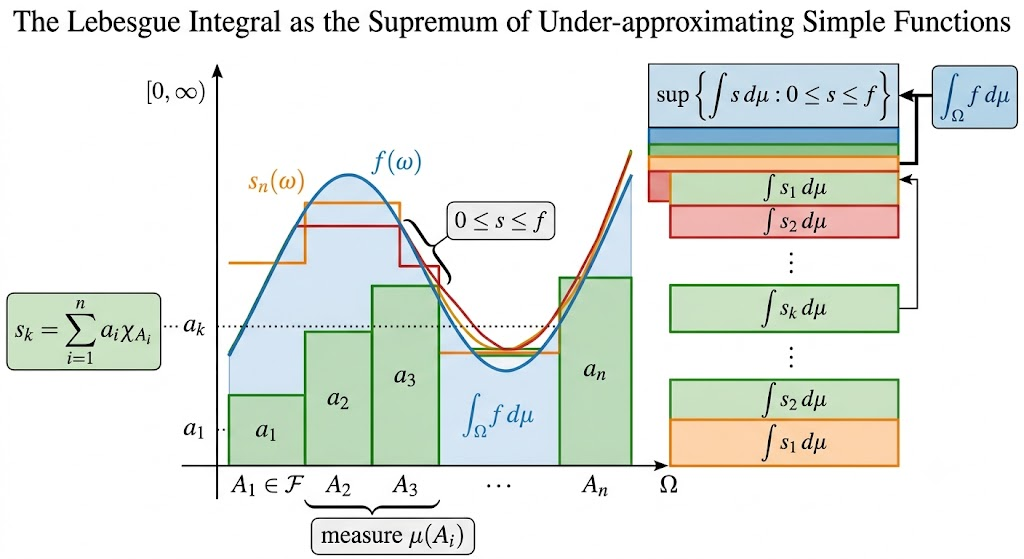
\includegraphics[width=\linewidth]{images/Legsgue-integral.jpg}
        \end{center}
    \end{columns}

    \vspace{0.3cm}
    \begin{alertblock}{Key Fact}
        Monotonicity is the \textbf{engine} behind Markov's and Tchebychev's inequalities.
    \end{alertblock}
\end{frame}

% =================== SLIDE 8: L^p SPACES ===================
\begin{frame}{$L^p$ Spaces}
    \begin{definition}[$L^p$ Space]
        For $1 \leq p < \infty$, the \textbf{Lebesgue space} $L^p(\Omega, \mu)$ is:
        \[
            L^p(\Omega, \mu) = \left\{f \text{ measurable} : \int_\Omega |f|^p \, d\mu < \infty \right\}
        \]
        equipped with the \textbf{$L^p$ norm}:
        \[
            \|f\|_p = \left(\int_\Omega |f|^p \, d\mu\right)^{1/p}.
        \]
    \end{definition}

    \vspace{0.3cm}
    \begin{block}{Intuition}
        \begin{itemize}
            \item $f \in L^1$: the function is ``absolutely integrable.''
            \item $f \in L^2$: the function has ``finite energy'' — this is the natural setting for Tchebychev.
        \end{itemize}
    \end{block}
\end{frame}

% ===================================================================
%                    SECTION: MARKOV'S INEQUALITY
% ===================================================================
\section{Markov's Inequality}

% =================== SLIDE 9: MARKOV STATEMENT ===================
\begin{frame}{Markov's Inequality — Statement}
    The starting point for Tchebychev is this simpler result:

    \begin{theorem}[Markov's Inequality]
        Let $f: \Omega \to [0, \infty]$ be a non-negative measurable function on $(\Omega, \mathscr{F}, \mu)$. For any $\alpha > 0$:
        \[
            \boxed{\mu\big(\{f \geq \alpha\}\big) \leq \frac{1}{\alpha} \int_\Omega f \, d\mu}
        \]
    \end{theorem}

    \vspace{0.3cm}
    \begin{alertblock}{In Words}
        The ``size'' of the set where $f$ is large is controlled by the integral of $f$.

        \vspace{0.2cm}
        \textit{Large values cannot occur on a large set if the integral is finite.}
    \end{alertblock}
\end{frame}

% =================== SLIDE 10: MARKOV PROOF ===================
\begin{frame}{Markov's Inequality — Proof}
    \begin{proof}
        Let $A = \{f \geq \alpha\} = \{\omega \in \Omega : f(\omega) \geq \alpha\}$.

        \vspace{0.3cm}
        \textbf{Step 1:} Since $f \geq 0$, restricting the domain of integration only decreases the integral:
        \[
            \int_\Omega f \, d\mu \geq \int_A f \, d\mu.
        \]

        \textbf{Step 2:} On the set $A$, we know $f(\omega) \geq \alpha$, so:
        \[
            \int_A f \, d\mu \geq \int_A \alpha \, d\mu = \alpha \cdot \mu(A).
        \]

        \textbf{Step 3:} Combining:
        \[
            \int_\Omega f \, d\mu \geq \alpha \cdot \mu(A) \implies \mu(A) \leq \frac{1}{\alpha}\int_\Omega f \, d\mu.
        \]
    \end{proof}

    \textit{We used only: monotonicity of the integral and the definition of $A$.}
\end{frame}

% ===================================================================
%                    SECTION: TCHEBYCHEV'S INEQUALITY
% ===================================================================
\section{Tchebychev's Inequality}

% =================== SLIDE 11: TCHEBYCHEV STATEMENT ===================
\begin{frame}{Tchebychev's Inequality — Statement}
    \begin{theorem}[Tchebychev's Inequality]
        Let $(\Omega, \mathscr{F}, \mu)$ be a finite measure space and $f \in L^2(\Omega, \mu)$.

        \vspace{0.2cm}
        Define the mean: $\displaystyle\bar{f} = \frac{1}{\mu(\Omega)} \int_\Omega f \, d\mu$.

        \vspace{0.2cm}
        Then for any $\lambda > 0$:
        \[
            \boxed{\mu\big(\{\omega : |f(\omega) - \bar{f}| \geq \lambda\}\big) \leq \frac{1}{\lambda^2} \int_\Omega |f - \bar{f}|^2 \, d\mu}
        \]
    \end{theorem}

    \vspace{0.3cm}
    \begin{block}{In Words}
        The measure of the set where $f$ deviates from its mean by at least $\lambda$ is bounded by the \textbf{variance} divided by $\lambda^2$.
    \end{block}
\end{frame}

% =================== SLIDE 12: TCHEBYCHEV PROOF ===================
\begin{frame}{Tchebychev's Inequality — Proof}
    \begin{proof}
        \textbf{Step 1:} Define $g = |f - \bar{f}|^2$. Note that $g \geq 0$ and $g$ is measurable.

        \vspace{0.3cm}
        \textbf{Step 2:} Observe the equivalence of level sets:
        \[
            |f - \bar{f}| \geq \lambda \iff |f - \bar{f}|^2 \geq \lambda^2 \iff g \geq \lambda^2.
        \]

        \vspace{0.3cm}
        \textbf{Step 3:} Apply Markov's inequality to $g$ with threshold $\lambda^2$:
        \[
            \mu(\{g \geq \lambda^2\}) \leq \frac{1}{\lambda^2} \int_\Omega g \, d\mu.
        \]

        \vspace{0.3cm}
        \textbf{Step 4:} Substitute back:
        \[
            \mu(\{|f - \bar{f}| \geq \lambda\}) \leq \frac{1}{\lambda^2} \int_\Omega |f - \bar{f}|^2 \, d\mu = \frac{\|f - \bar{f}\|_2^2}{\lambda^2}.
        \]
    \end{proof}
\end{frame}

% =================== SLIDE 13: WHY IT WORKS ===================
\begin{frame}{Why Does the Proof Work?}
    The proof relies on exactly \textbf{two} analytic facts:

    \vspace{0.4cm}
    \begin{block}{1. Monotonicity of the Lebesgue Integral}
        If $f \leq g$ a.e., then $\int f \, d\mu \leq \int g \, d\mu$.

        \vspace{0.2cm}
        \textit{This is what makes Markov's inequality true.}
    \end{block}

    \vspace{0.3cm}
    \begin{block}{2. Measurability of Level Sets}
        If $f$ is measurable, then $\{|f| \geq \lambda\} \in \mathscr{F}$ for every $\lambda > 0$.

        \vspace{0.2cm}
        \textit{This ensures $\mu(\{|f| \geq \lambda\})$ is well-defined.}
    \end{block}

    \vspace{0.4cm}
    \begin{center}
        \textbf{No assumptions} on the structure of $\Omega$, the form of $\mu$, or the shape of $f$ are needed.
    \end{center}
\end{frame}

% =================== SLIDE: STATISTICAL FORM (k*sigma) ===================
\begin{frame}{Statistical Form: $k\sigma$ Version}
    In statistics, Tchebychev is often stated using $k$ standard deviations:

    \begin{block}{$k\sigma$ Form}
        Let $X$ have mean $\mu$ and standard deviation $\sigma > 0$. For any $k > 0$:
        \[
            P(|X - \mu| \geq k\sigma) \leq \frac{1}{k^2}
        \]
    \end{block}

    \begin{exampleblock}{Example: Exam Scores}
        A class has mean score $\mu = 70$ and standard deviation $\sigma = 10$.

        \vspace{0.2cm}
        \textbf{What fraction of students can score outside $[50, 90]$?}

        \vspace{0.2cm}
        Here $|X - 70| \geq 20 = 2\sigma$, so $k = 2$:
        \[
            P(|X - 70| \geq 20) \leq \frac{1}{2^2} = \frac{1}{4} = 25\%.
        \]
        At least \textbf{75\%} of students score between 50 and 90.
    \end{exampleblock}
\end{frame}

% =================== SLIDE: RAW DISTANCE VERSION ===================
\begin{frame}{Statistical Form: Raw Distance Version}
    We can also state the bound directly in terms of the deviation $\lambda$:

    \begin{block}{Raw Distance Form}
        Let $X$ have mean $\mu$ and variance $\sigma^2$. For any $\lambda > 0$:
        \[
            P(|X - \mu| \geq \lambda) \leq \frac{\sigma^2}{\lambda^2}
        \]
    \end{block}

    \begin{exampleblock}{Example: Delivery Times}
        A courier's delivery time has mean $\mu = 30$ min and variance $\sigma^2 = 25$ min$^2$.

        \vspace{0.2cm}
        \textbf{What is the chance of deviating by more than 15 minutes?}

        \vspace{0.2cm}
        Set $\lambda = 15$:
        \[
            P(|X - 30| \geq 15) \leq \frac{25}{15^2} = \frac{25}{225} = \frac{1}{9} \approx 11.1\%.
        \]
        At least \textbf{88.9\%} of deliveries arrive between 15 and 45 minutes.
    \end{exampleblock}
\end{frame}

% ===================================================================
%                    SECTION: APPLICATIONS
% ===================================================================
\section{Applications}

% =================== SLIDE 15: APPLICATIONS ===================
\begin{frame}{Applications of Tchebychev's Inequality}
    Tchebychev's inequality is applied in the following areas:

    \vspace{0.2cm}
    \begin{itemize}
        \item \textbf{Convergence Theory:} $L^p$ convergence implies convergence in measure.
        \item \textbf{Weak Law of Large Numbers:} Sample averages converge to the mean.
        \item \textbf{Approximation Theory:} Bernstein's proof of the Weierstrass theorem.
        \item \textbf{Fourier Analysis:} $L^2$ convergence of partial sums implies convergence in measure.
        \item \textbf{Ergodic Theory:} Convergence of ergodic averages via $L^2$ bounds.
        \item \textbf{PDE \& Sobolev Spaces:} Controlling level sets via Sobolev norms.
        \item \textbf{Spectral Theory:} Bounding spectral measure for self-adjoint operators.
    \end{itemize}

    \vspace{0.3cm}
    \textit{In each case: \textbf{integral estimates} $\longrightarrow$ \textbf{pointwise control}.}
\end{frame}

% ===================================================================
%                    SECTION: SHARPNESS
% ===================================================================
\section{Sharpness}

% =================== SLIDE 16: SHARPNESS ===================
\begin{frame}{Sharpness of Tchebychev's Inequality}
    \begin{alertblock}{The bound is tight!}
        For any $\lambda > 0$, there exists a measurable function for which \textbf{equality} holds.
    \end{alertblock}

    \vspace{0.2cm}
    \begin{exampleblock}{Extremal Example}
        Let $\Omega = \{-1, 0, 1\}$ with $\mu(\{-1\}) = \mu(\{1\}) = \frac{1}{2k^2}$, \ $\mu(\{0\}) = 1 - \frac{1}{k^2}$.

        \vspace{0.2cm}
        Define $f(\omega) = \omega$. Then $\bar{f} = 0$, $\sigma^2 = 1/k^2$, and:
        \[
            \mu(\{|f| \geq 1\}) = \frac{1}{k^2} = \frac{\sigma^2}{\lambda^2}. \quad \checkmark
        \]
    \end{exampleblock}

    \vspace{0.2cm}
    \textit{Tighter bounds need extra assumptions (sub-Gaussian, log-concavity, etc.).}
\end{frame}

% ===================================================================
%                    SECTION: REFERENCES
% ===================================================================
\section{References}

% =================== SLIDE 24: REFERENCES ===================
\begin{frame}{References}
    \begin{thebibliography}{9}
        \bibitem{tchebychev1867}
            P. L. Tchebychev (1867).
            \newblock \emph{Des valeurs moyennes}.
            \newblock Liouville's Journal, 2(12), 177-184.

        \bibitem{rudin}
            W. Rudin (1987).
            \newblock \emph{Real and Complex Analysis} (3rd ed.).
            \newblock McGraw-Hill.

        \bibitem{folland}
            G. B. Folland (1999).
            \newblock \emph{Real Analysis: Modern Techniques and Their Applications} (2nd ed.).
            \newblock Wiley.

        \bibitem{stein}
            E. M. Stein and R. Shakarchi (2005).
            \newblock \emph{Real Analysis}.
            \newblock Princeton University Press.
    \end{thebibliography}
\end{frame}

% =================== SLIDE 25: THANK YOU ===================
\begin{frame}{}
    \begin{center}
        \Huge \textcolor{blue}{Thank You}

        \vspace{0.5cm}

        \vspace{0.5cm}
        \normalsize Questions?
    \end{center}
\end{frame}

\end{document}